%=========================================================================
% Start of activity on piece wise defined functions and max/min
%=========================================================================
\preClass{Introduction to Piece-wise Defined Functions}

\begin{problem}
\item The graph of a function, $g$, is shown shown below:

  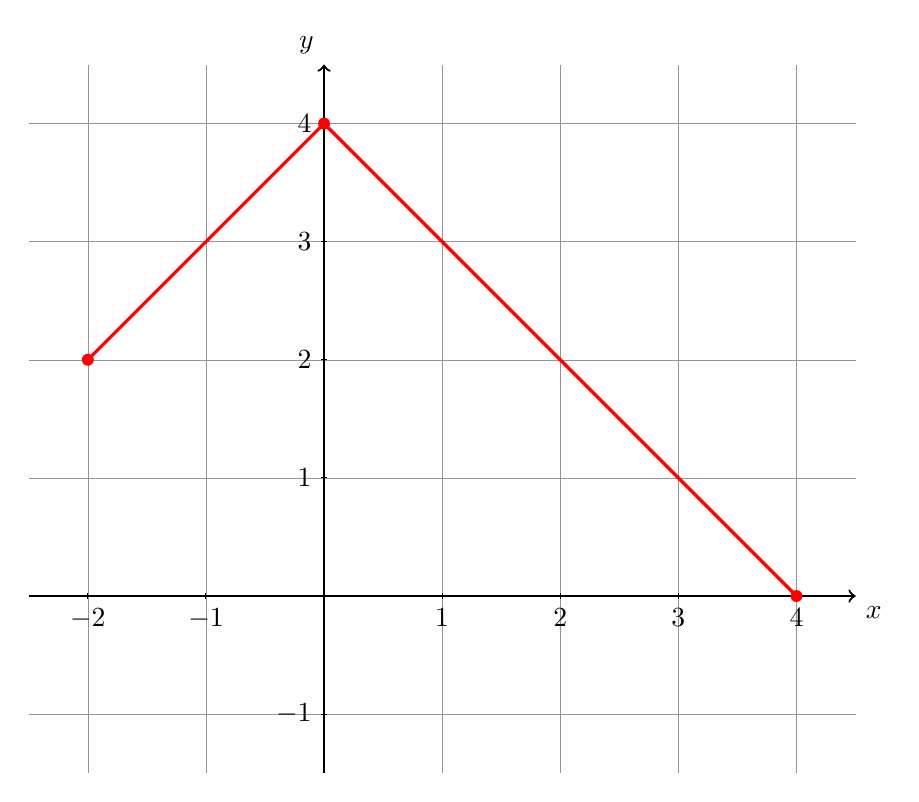
\begin{tikzpicture}[y=1.5cm, x=1.5cm,font=\sffamily]
    % ticks
    \draw[step = 1, gray, very thin,opacity=0.85] (-2.5, -1.5) grid ( 4.5, 4.5);
 	% axis
	\draw[thick,->] (-2.5,0) -- coordinate (x axis mid) (4.5,0) 
          node[anchor = north west] {$x$};
    \draw[thick,->] (0,-1.5) -- coordinate (y axis mid) (0,4.5) 
          node[anchor = south east] {$y$};
    \foreach \y in {-1,1,2,3,4} {
      \draw (1pt, \y) -- (-1pt, \y) node[anchor = east] {$\y$};
    }
    \foreach \x in {-2,-1,1,2,3,4} {
      \draw (\x,1pt) -- (\x,-1pt) node[anchor = north] {$\x$};
    }
    % Draw the function
    \draw [red, very thick] plot coordinates {(-2,2) (0,4) (4,0)};
    \fill[red] (-2, 2) circle [radius=0.5ex];
    \fill[red] ( 0, 4) circle [radius=0.5ex];
    \fill[red] ( 4,0) circle [radius=0.5ex];
  \end{tikzpicture}

  \begin{subproblem}
  \item Determine the domain and range of the function.
    \vfill
  \item Determine the formula for the function if $x\geq -2$ and
    $x<0$.
    \vfill
  \item Determine the formula for the function if $x> 0$ and
    $x\leq 4$.
    \vfill
  \item For what values of $x$ is the function increasing?
    \vspace{2em}
  \item For what values of $x$ is the function decreasing?
    \vspace{2em}
  \end{subproblem}

\end{problem}


\actTitle{Piece-wise Defined Functions}
\begin{problem}
\item A piece of metal is initially at 20C. It is placed in a hot
  furnace for twenty-five minutes, and its temperature is raised to
  200C. It is then removed from the oven and placed in cold water and
  cooled to room temperature.. After five minutes it is placed back
  into the furnace, and the process is repeated three times. Make a
  sketch of the graph of the temperature of the piece of metal on the
  axes below.

    \hspace{-7em}
    \begin{tikzpicture}[y=0.03cm, x=0.14cm,font=\sffamily]
        % bounds
        \def\lowX{-0.5}
        \pgfmathtruncatemacro\startX{round(0.5+\lowX)}
        \pgfmathsetmacro\nextXValue{int(\startX+1)}
        \def\highX{100.5}
        \def\lowY{-0.5}
        \def\highY{220.0}
        \pgfmathsetmacro\nextYValue{int(\lowY+1)}
        % ticks
        \draw[xstep = 10,ystep=50, gray, very thin,dashed,opacity=0.85] (\lowX, \lowY) grid ( \highX,\highY);
      % axis
      \draw[thick,->] (\lowX,0) -- coordinate (x axis mid) (\highX,0) node[anchor = north west] {Time (Min)};
        \draw[thick,->] (0,\lowY) -- coordinate (y axis mid) (0,\highY) node[anchor = north east] {Temp. (C)};
        \foreach \y in {50,100,...,\highY} {
          \draw (1pt, \y) -- (-1pt, \y) node[yshift=-6,xshift=-1,anchor=east] {$\y$};
        }
        \foreach \x in {10,20,...,\highX} {
          \draw (\x,1pt) -- (\x,-1pt) node[yshift=-5,xshift=-1,anchor=east] {$\x$};
        }
        %\draw (0,5.5) node [anchor=south] {Comparing Shifted Functions};
      \end{tikzpicture}

      \begin{subproblem}
      \item What is the range and domain of the function?
        \vfill
      \item Determine the values of the time where the function is
        increasing.
        \vfill
      \item Determine the values of the time where the function is
        decreasing.  
        \vfill
      \end{subproblem}

      \clearpage
\item The questions below refer to the function whose graph is given
  below.

  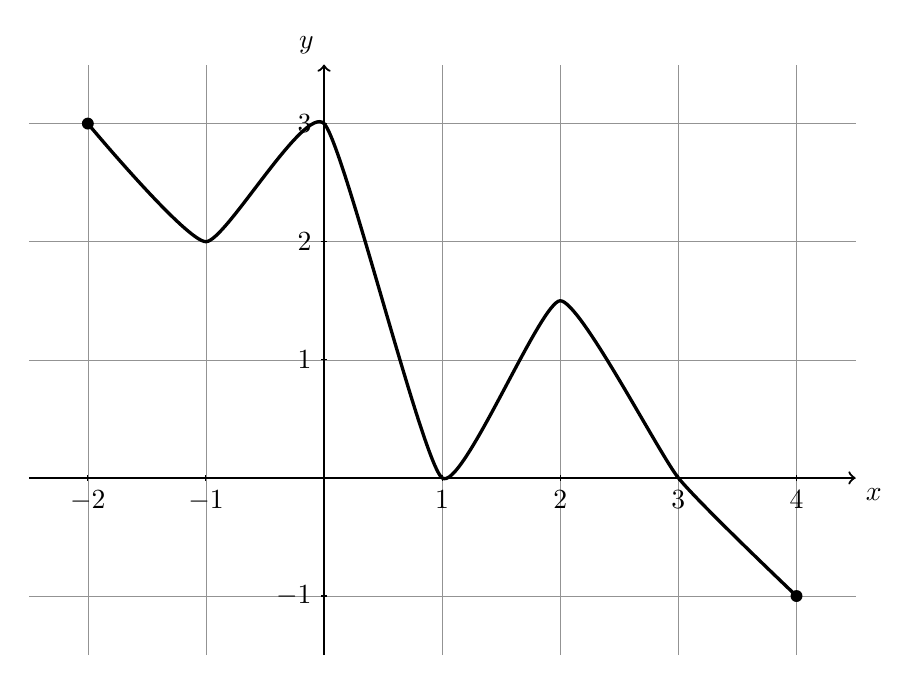
\begin{tikzpicture}[y=1.5cm, x=1.5cm,font=\sffamily]
    % ticks
    \draw[step = 1, gray, very thin,opacity=0.85] (-2.5, -1.5) grid ( 4.5, 3.5);
 	% axis
	\draw[thick,->] (-2.5,0) -- coordinate (x axis mid) (4.5,0) 
          node[anchor = north west] {$x$};
    \draw[thick,->] (0,-1.5) -- coordinate (y axis mid) (0,3.5) 
          node[anchor = south east] {$y$};
    \foreach \y in {-1,1,2,3} {
      \draw (1pt, \y) -- (-1pt, \y) node[anchor = east] {$\y$};
    }
    \foreach \x in {-2,-1,1,2,3,4} {
      \draw (\x,1pt) -- (\x,-1pt) node[anchor = north] {$\x$};
    }
    % Draw the function
    \draw [black, very thick] plot [smooth, tension=0.3] coordinates {
      (-2,3) (-1,2) (0,3) (1,0) (2,1.5) (3,0) (4,-1)};
    \fill (-2, 3) circle [radius=0.5ex];
    \fill ( 4,-1) circle [radius=0.5ex];
  \end{tikzpicture}

  \begin{subproblem}
    \item Determine the domain and range of the function.
      \vfill
    \item Determine the values of $x$ where the function is
      increasing.
      \vfill
    \item Determine the values of $x$ where the function is
      decreasing.
      \vfill
  \end{subproblem}

  \clearpage

\item Make sketch of the graph of the function
  \begin{eqnarray*}
    \mathrm{Harold}(x) & = & \left\{
                             \begin{array}{l@{\hspace{3em}}rcccl}
                               \frac{1}{2}(x+2) & -2 & \leq & x & < &  0, \\
                               4-x^2            &  0 &   <  & x & < &  2, \\
                               -2(x-2)          &  2 & \leq & x & < & 4.
                             \end{array}
                             \right.
  \end{eqnarray*}
  Determine the domain and range of the function. Determine where the
  function is increasing. Also determine where it is decreasing.

    \begin{tikzpicture}[y=1.1cm, x=1.1cm,font=\sffamily]
        % bounds
        \def\lowX{-5.5}
        \pgfmathtruncatemacro\startX{round(0.5+\lowX)}
        \pgfmathsetmacro\nextXValue{int(\startX+1)}
        \def\highX{5.5}
        \def\lowY{-5.5}
        \def\highY{5.5}
        \pgfmathsetmacro\nextYValue{int(\lowY+1)}
        % ticks
        \draw[step = 1, gray, very thin,dashed,opacity=0.85] (\lowX, \lowY) grid ( \highX,\highY);
      % axis
      \draw[thick,->] (\lowX,0) -- coordinate (x axis mid) (\highX,0) node[anchor = north west] {$x$};
        \draw[thick,->] (0,\lowY) -- coordinate (y axis mid) (0,\highY) node[anchor = north east] {$y$};
        \foreach \y in {-5,-4,...,-1,1,2,...,\highY} {
          \draw (1pt, \y) -- (-1pt, \y) node[yshift=-6,xshift=-1,anchor=east] {$\y$};
        }
        \foreach \x in {-5,-4,...,-1,1,2,...,\highX} {
          \draw (\x,1pt) -- (\x,-1pt) node[yshift=-5,xshift=-1,anchor=east] {$\x$};
        }
        %\draw (0,5.5) node [anchor=south] {Comparing Shifted Functions};
      \end{tikzpicture}


\clearpage

\item Part of the graph of a function is given below. The function is
  even. Sketch the rest of the function. Determine the domain and
  range of the function.

    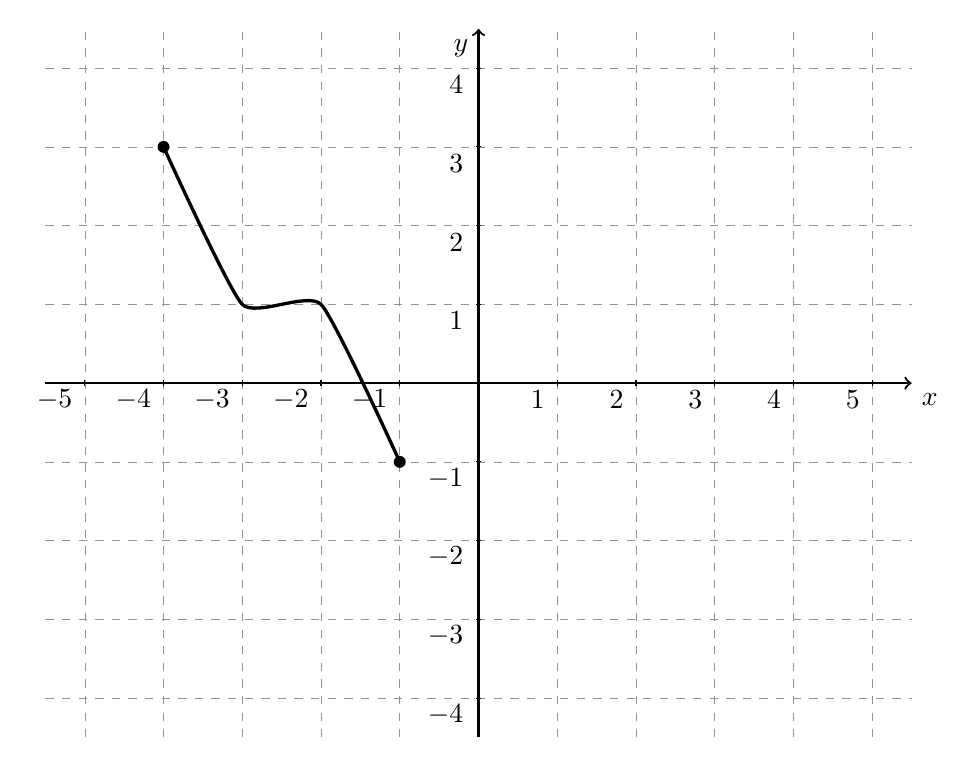
\begin{tikzpicture}[y=1.0cm, x=1.0cm,font=\sffamily]
        % bounds
        \def\lowX{-5.5}
        \pgfmathtruncatemacro\startX{round(0.5+\lowX)}
        \pgfmathsetmacro\nextXValue{int(\startX+1)}
        \def\highX{5.5}
        \def\lowY{-4.5}
        \def\highY{4.5}
        \pgfmathsetmacro\nextYValue{int(\lowY+1)}
        % ticks
        \draw[step = 1, gray, very thin,dashed,opacity=0.85] (\lowX, \lowY) grid ( \highX,\highY);
      % axis
      \draw[thick,->] (\lowX,0) -- coordinate (x axis mid) (\highX,0) node[anchor = north west] {$x$};
        \draw[thick,->] (0,\lowY) -- coordinate (y axis mid) (0,\highY) node[anchor = north east] {$y$};
        \foreach \y in {-4,-3,...,-1,1,2,...,\highY} {
          \draw (1pt, \y) -- (-1pt, \y) node[yshift=-6,xshift=-1,anchor=east] {$\y$};
        }
        \foreach \x in {-5,-4,...,-1,1,2,...,\highX} {
          \draw (\x,1pt) -- (\x,-1pt) node[yshift=-5,xshift=-1,anchor=east] {$\x$};
        }
        \draw [black, very thick] plot [smooth, tension=0.3] coordinates {
          (-4,3) (-3,1) (-2,1) (-1,-1)};
        \fill (-4, 3) circle [radius=0.5ex];
        \fill (-1,-1) circle [radius=0.5ex];

      \end{tikzpicture}

    \item Part of the graph of a function is given below. The function
      is odd. Sketch the rest of the function. Determine the domain
      and range of the function.

    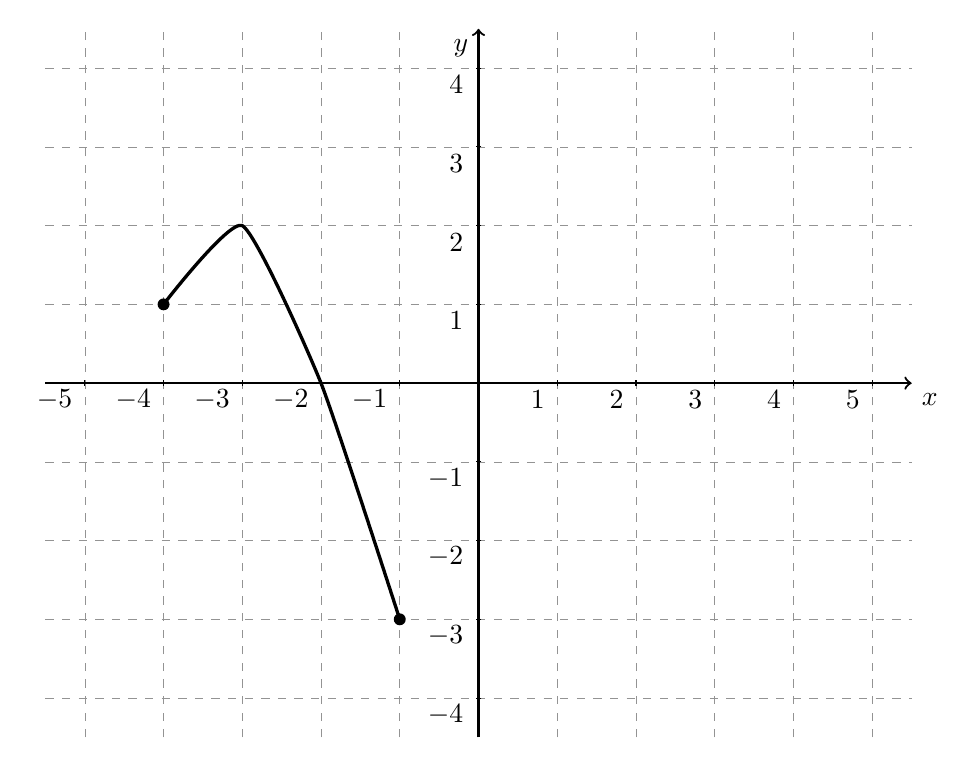
\begin{tikzpicture}[y=1.0cm, x=1.0cm,font=\sffamily]
        % bounds
        \def\lowX{-5.5}
        \pgfmathtruncatemacro\startX{round(0.5+\lowX)}
        \pgfmathsetmacro\nextXValue{int(\startX+1)}
        \def\highX{5.5}
        \def\lowY{-4.5}
        \def\highY{4.5}
        \pgfmathsetmacro\nextYValue{int(\lowY+1)}
        % ticks
        \draw[step = 1, gray, very thin,dashed,opacity=0.85] (\lowX, \lowY) grid ( \highX,\highY);
      % axis
      \draw[thick,->] (\lowX,0) -- coordinate (x axis mid) (\highX,0) node[anchor = north west] {$x$};
        \draw[thick,->] (0,\lowY) -- coordinate (y axis mid) (0,\highY) node[anchor = north east] {$y$};
        \foreach \y in {-4,-3,...,-1,1,2,...,\highY} {
          \draw (1pt, \y) -- (-1pt, \y) node[yshift=-6,xshift=-1,anchor=east] {$\y$};
        }
        \foreach \x in {-5,-4,...,-1,1,2,...,\highX} {
          \draw (\x,1pt) -- (\x,-1pt) node[yshift=-5,xshift=-1,anchor=east] {$\x$};
        }
        \draw [black, very thick] plot [smooth, tension=0.3] coordinates {
          (-4,1) (-3,2) (-2,-0) (-1,-3)};
        \fill (-4, 1) circle [radius=0.5ex];
        \fill (-1,-3) circle [radius=0.5ex];

      \end{tikzpicture}

      \clearpage

    \item A small company builds a set of solar panels. The amount of
      electricity produced is proportional to the intensity of sun
      light. When the sunlight is bright, 100,000 lux, the system
      produces 4,000 watts. On one day of operation there is a good
      deal of cloud cover, and the amount of sunlight varies linearly
      from 6am to noon from 0 lux to 50,000 lux. After noon it varies
      linearly to 0 lux at 6pm. On the second day the cycle repeats,
      but the maximum amount of light is 100,000 lux. Determine the
      amount of power produced by the panel at any time during the two
      days. (Include night time!)

      \vfill

\end{problem}

\postClass

\begin{problem}
\item Briefly state two ideas from today's class.
  \begin{itemize}
  \item 
  \item 
  \end{itemize}
\item 
  \begin{subproblem}
    \item
  \end{subproblem}
\end{problem}


%%% Local Variables:
%%% mode: latex
%%% TeX-master: "../labManual"
%%% End:

